\documentclass{article}
\usepackage{amsmath,amsfonts,amssymb}
\usepackage{graphicx}
\usepackage{tikz}
\usetikzlibrary{arrows}
\usepackage[margin=1in]{geometry}
\begin{document}

\title{Carrier Modulation: Fourier Transform and Spectrum Analysis}
\author{}
\maketitle

\section*{Problem Statement}

For \( x(t) = B \, \text{sinc}(Bt) \cos(2\pi f_c t) \) where \( f_c \gg 1 \) and \( B = 20 \, \text{MHz} \), determine:

\begin{itemize}
  \item[(a)] Express the Fourier transform (FT) of \( x(t) \).
  \item[(b)] Draw the spectrum (only \( |X(f)| \)) and show the values on both \( x \)- and \( y \)-axes.
\end{itemize}

\section*{Solutions}

\subsection*{Fourier Transform of \( x(t) \)}

We are given the time-domain signal \( x(t) \) as:

\[
x(t) = B \, \text{sinc}(Bt) \cos(2\pi f_c t)
\]

To find its Fourier Transform \( X(f) \), we will utilize two main properties of the Fourier Transform: modulation and convolution.

\subsubsection*{Step 1: Fourier Transform of the sinc Function}

First, we consider the Fourier Transform of the sinc function \( \text{sinc}(Bt) \). By standard Fourier Transform tables, we know that:

\[
\mathcal{F}\{\text{sinc}(Bt)\} = \text{rect}\left(\frac{f}{B}\right)
\]

Here \( \text{rect}(x) \) is the rectangular function, defined as:

\[
\text{rect}(x) = 
\begin{cases} 
1, & \text{if } |x| < \frac{1}{2} \\
0, & \text{otherwise}
\end{cases}
\]

This rectangular function in the frequency domain has a width of \( 2B \).

\subsubsection*{Step 2: Modulation}

Multiplying \( \text{sinc}(Bt) \) by \( \cos(2\pi f_c t) \) in the time domain corresponds to frequency modulation in the frequency domain. This results in the creation of sidebands located at \( f_c \) and \( -f_c \).

The Fourier Transform \( X(f) \) can be mathematically represented as:

\[
X(f) = \frac{B}{2} \left( \text{rect}\left(\frac{f - f_c}{B}\right) + \text{rect}\left(\frac{f + f_c}{B}\right) \right)
\]

In this formula, \( \text{rect}\left(\frac{f - f_c}{B}\right) \) signifies the part of the spectrum that has been shifted to \( f_c \), and \( \text{rect}\left(\frac{f + f_c}{B}\right) \) represents the part shifted to \( -f_c \).

The division by 2 occurs because the original spectrum of \( \text{sinc}(Bt) \) is effectively being split between the two sidebands, each receiving half of the total spectral energy.


\subsection*{Spectrum \( |X(f)| \)}

\subsubsection*{Drawing the Spectrum}
I am unsure if there needs to be a division by $2\pi$ so I included both options. \newline\newline
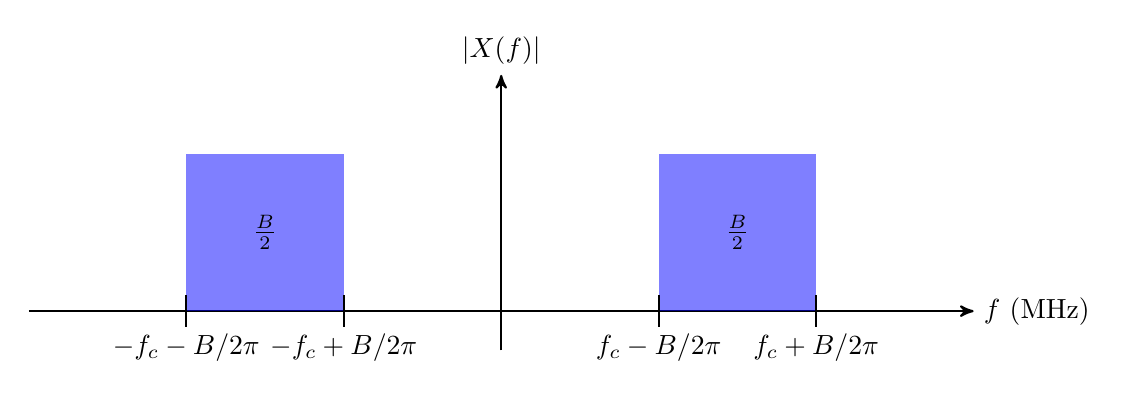
\begin{tikzpicture}[>=stealth']
    % Draw x-axis and y-axis
    \draw[thick,->] (-6,0) -- (6,0) node[right] { \( f \) (MHz)};
    \draw[thick,->] (0,-0.5) -- (0,3) node[above] { \( |X(f)| \) };

    % Draw rectangles for frequency components
    \fill[blue,opacity=0.5] (-4,0) rectangle (-2,2);
    \fill[blue,opacity=0.5] (2,0) rectangle (4,2);

    % Label frequency components
    \node at (-3,1) { \( \frac{B}{2} \) };
    \node at (3,1) { \( \frac{B}{2} \) };

    % Label frequency values
    \draw[thick] (-2,-0.2) -- (-2,0.2) node[below=10pt] { \( -f_c + B/2\pi \) };
    \draw[thick] (-4,-0.2) -- (-4,0.2) node[below=10pt] { \( -f_c - B/2\pi \) };
    \draw[thick] (2,-0.2) -- (2,0.2) node[below=10pt] { \( f_c - B/2\pi \) };
    \draw[thick] (4,-0.2) -- (4,0.2) node[below=10pt] { \( f_c + B/2\pi \) };
\end{tikzpicture}
\newline
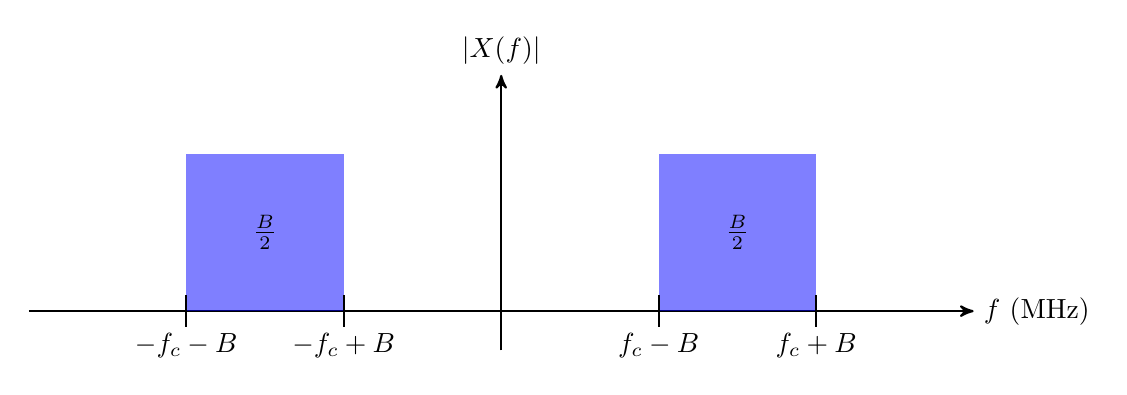
\begin{tikzpicture}[>=stealth']
    % Draw x-axis and y-axis
    \draw[thick,->] (-6,0) -- (6,0) node[right] { \( f \) (MHz)};
    \draw[thick,->] (0,-0.5) -- (0,3) node[above] { \( |X(f)| \) };

    % Draw rectangles for frequency components
    \fill[blue,opacity=0.5] (-4,0) rectangle (-2,2);
    \fill[blue,opacity=0.5] (2,0) rectangle (4,2);

    % Label frequency components
    \node at (-3,1) { \( \frac{B}{2} \) };
    \node at (3,1) { \( \frac{B}{2} \) };

    % Label frequency values
    \draw[thick] (-2,-0.2) -- (-2,0.2) node[below=10pt] { \( -f_c + B \) };
    \draw[thick] (-4,-0.2) -- (-4,0.2) node[below=10pt] { \( -f_c - B \) };
    \draw[thick] (2,-0.2) -- (2,0.2) node[below=10pt] { \( f_c - B \) };
    \draw[thick] (4,-0.2) -- (4,0.2) node[below=10pt] { \( f_c + B \) };
\end{tikzpicture}
\end{document}
